\section{Algoritme til detektering og adskillelse af aktiviteter}

For at kunne adskille gang, løb og cykling benyttes et accelerometer og et gyroskop som er beskrevet i \secref{LSM9DS1}\fxnote{opg: tjek op på denne reference}. Herunder vil gyroskopet blive benyttet til at detektere cykling, mens løb og gang detekteres ved brug af accelerometeret. For at kunne detektere og adskille disse aktiviteter, behandles inputtet fra sensorerne gennem forskellig signalbehandling, hvorefter algoritmer afgør om de pågældende signaler repræsenterer gang, løb, cykling eller ingen aktivitet.

\subsection{Design}
\subsubsection{Cykling}
Data fra gyroskopets z-akse skal signalbehandles, førend en algoritme kan detektere og adskille aktiviteterne. Første step i denne signalbehandling er at udføre en Fast Fourier Transform (FFT) over to sekunders sampling. Dette medfører at signalets magnitude og dets tilhørende frekvenser kommer til udtryk, hvoraf andet step indledes. Dette step finder den maksimale magnitude med tilhørende frekvens. Tredje step består af to integraler, første integrale integrer FFT'en fra den frekvens hvor den største magnitude befandt sig $\pm 1$Hz. Andet integrale integrer FFT'en fra 1 til 20 Hz. Disse integraler indleder fjerde og sidste step, som omregner hvor stor en procentdel første integrale udgør af signalets totale energi. \\
Resultatet af ovenstående signalbehandling medfører at der opstilles et udtryk for signalets spredning af energi. Det gør sig gældende at cykling har en spredning af energi fordelt nært frekvensen med den største amplitude. Data fra gyroskopets z-akse vedrørende cykling blev for alle forsøgspersoner, behandlet med ovenstående metode. Dette resulterede i at 84,2\% til 88,4\% af energien lå $\pm 1$Hz omkring den fundne frekvens. Følgende blev ligeledes behandlet for gang og løb, for at sikre disse ikke havde samme spredning i frekvensområdet, hvormed en mulig tærskelværdi til detektering af cykling, kan fastsættes.  Dette resulterede i at ved gang befandt energien omkring den fundne frekvens sig mellem 47,2\% til 55,4\% og ved løb befandt energien omkring den fundne frekvens sig mellem 42\% til 50,6\%. \\
Resultatet af at energien omkring den fundne frekvens med den største amplitude er $\approx$30\% større ved cykling end ved gang og løb, fastsættes tærskelværdien til 70\%. For at detektere cykling skal outputtet fra databehandlingen være større end 70\%.

\begin{figure}[H]
	\centering
	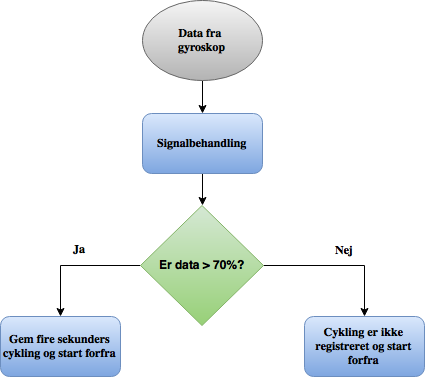
\includegraphics[scale=0.6]{figures/cDesign/algoritme_cykling.png}
	\caption{På figuren ses et flowchart som gennemgår algoritmen vedrørende detektering af cykling.}
	\label{fig:algoritme_cykling}
\end{figure}
 
Ovenstående figur repræsenterer algoritmen for detektering af cykling. Hvis cykling detekteres skal en counter starte og først stoppe når cykling ikke længere detekteres. Når counteren stopper gemmes varigheden af counteren i et array tilhørende udført cykling. Hvis cykling ikke detekteres skal gyroskopet gå i LPM i 10 sekunder før algoritmen køres igen. 

\subsection{Implementering}
\subsubsection{Cykling}

\subsection{Design}



%%%%% Behandling af gyro data %%%%%
\begin{enumerate}
	\item Gyro sleep i 10 sek - vækkes af interrupt.
	\item Opsaml data i 2 sek.
	\item FFT af rå data.
	\item Find max y af (1)
	\item Find arrayplads (x) for (2) \textrightarrow omregn til Hz : (2)/(antal samples/fs)
	\item Integrer (1) fra (3)-1 til (3)+1.
	\item Integrer (1) over 20 samples.
	\item Udregn hvor stor en del af (5) som består af (4) \textrightarrow (4)/(5)*100 = anden i \%.
	\item Threshold: cykling = > 70\% \textrightarrow optag og gem i flash, < 70\% \textrightarrow optag accelerometer. 
\end{enumerate}

%Pseudo kode  (Flowcharts)
%Timers, interrupts, clocks, powermodes
%Clocks: tæller tid...
%interrupt: start/stop ny funktion
%Databehandling/filtrering
%Tjek om det er cykling - hvis ja, start gyro
%Delay → send data til GAP central hvert 15. minut

